\presub
\subsection{Finding Frequent Items} \postsub
\label{sub:findfreq}

\ppp{Data Structure (Figure \ref{draw:freq}):}
\aname{} for finding frequent items only uses a min-heap. No filter is necessary since there is no need to remove duplicates. Here the interest is the frequency, \ie, the number of appearances of an item. 

%%
{
\color{reviewD}
\ppp{Insertion:}
The insertion process of the min-heap is exactly the same as that of our framework (see Section \ref{sub:findinterest}).
%The difference is that there is no Bloom filter.
%Given an incoming item, we check whether it is in the min-heap. If the item is in the min-heap, we increment the corresponding frequency by one. Otherwise, if the min-heap is not full, we insert the item into the min-heap. If the min-heap is full, we use the PRI technique.
}

%%
{
\color{reviewD}
\ppp{Report:}
The report process of finding frequent items is exactly the same as that of our framework (see Section \ref{sub:findinterest}).
%To report the items above a given threshold $\mathcal{T}$, we traverse the min-heap to return the items with frequencies larger than $\mathcal{T}$.
}
%
%\begin{figure}[htbp]
%	\centering
%	\prefig
%	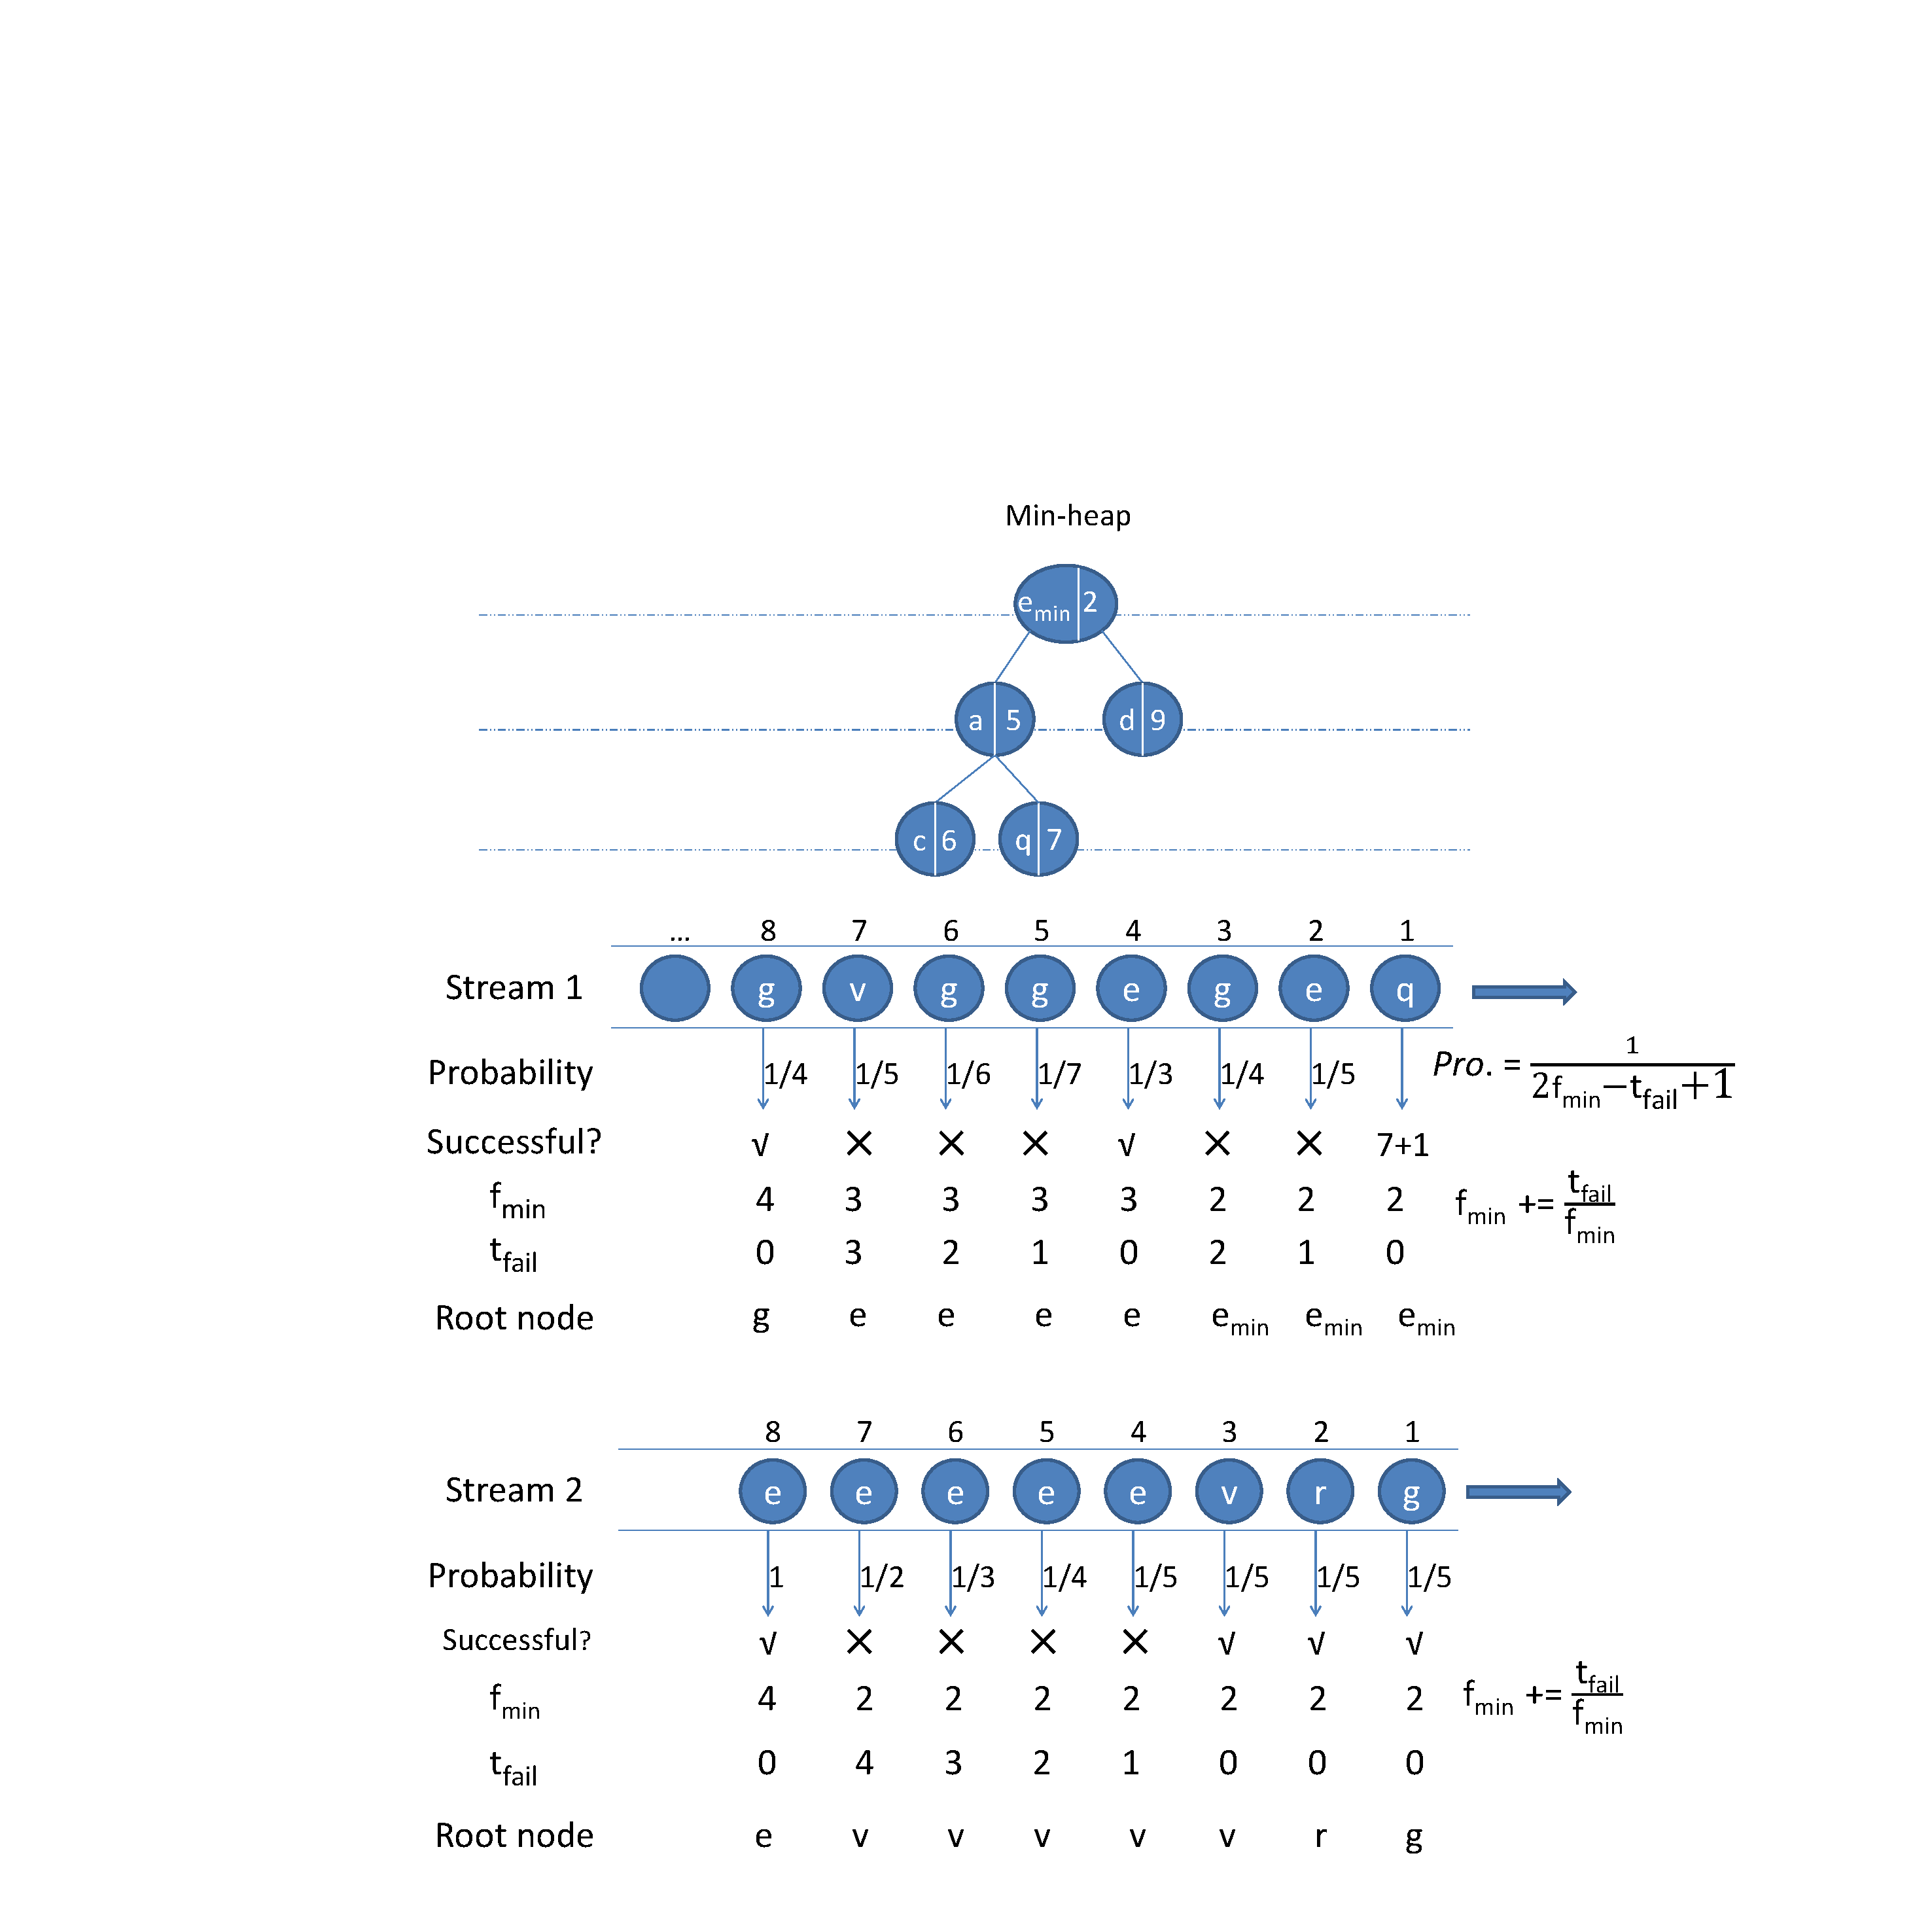
\includegraphics[width=0.5\textwidth]{GraphPPT/example_freq}
%	\prefigcaption \vvv\vvv
%	\caption{\aname{} for finding frequent items.
%
%	\label{draw:freq}
%	\postfig \vvv\vvv
%\end{figure}


%%
%\ppp{Example 1 (Figure~\ref{draw:freq}):}
%%
%Given a data stream (stream 1): $q,e,g,e,g,g,v$ \lar{,g}, for the first incoming item $q$, we increment the frequency of $q$ in the min-heap by one.
%
%For the following two items $e$ and $g$, replacements fail, and thus $t_{fail}$ is incremented to 1 and then 2. The probability increases to 1/3 for the fourth item $e$.
%
%Then $e_{min}$ is successfully replaced by the fourth item $e$ in the root node, and the frequency $f_{min}$ is incremented by $\frac{t_{fail}}{f_{min}}=1$, from 2 to 3, and  $t_{fail}$ is reset to 0.
%
%Since the actual frequency of item $e$ is 2 at present but we record it as 3, the frequency is slightly overestimated.
%
%Then the following 3 items ($g$, $g$, $v$) arrive and replace $e$ with probabilities 1/7, 1/6, and 1/5, but all fail. 
%
%Finally, the eighth item $g$ successfully replaces $e$ and the frequency $f_{min}$ is incremented from 3 to 4, which is exactly the frequency of item $g$ by now in data stream 1. 

%%
%\ppp{Example 2 (Figure \ref{draw:freq}):}
%
%Given another data stream (stream 2): $g, r, v, e, e, e, e, e, e$, \lar{one redundant e} suppose that each of the first three items successfully replaces the root node with the same probability of 1/5, and increments the frequency $f_{min}$ by $\frac{t_{fail}}{f_{min}}(=0)$ each time. \xy{$t_{fail}$ of the last e should be 0}
%
%Then item $e$ arrives five times in succession. 
%
%After four unsuccessful replacements with probabilities 1/5, 1/4, 1/3, and 1/2, the eighth item $e$ replaces item $v$ in the root node with probability 1, and increments the frequency $f_{min}$ by $\frac{t_{fail}}{f_{min}}(=2)$, from 2 to 4. 
%
%The frequency $f_{min}$ is slightly underestimated, since item $e$ has appeared 5 times in the data stream by now. 
%
%The first three replacements are wrong, but do not bring a large error to the final value of $f_{min}$. 

%%
%From the two examples, we see that in our algorithm, the frequency $f_{min}$ might be overestimated or underestimated.
%
%Fortunately, an item might be overestimated at first, but it could be underestimated later, and finally the estimate of the item is probably very close to its true value.
%
%%the average value of the estimator is almost accordant with the actual value, indicating a good unbiasedness of our algorithm. 
%
Moreover, successful replacement of infrequent items hardly impact the final result of $f_{min}$.

%
%%The algorithm is shown in Algorithm~\ref{alg:fre} in Appendix~\ref{sec:appendix}.
%The detailed description of the algorithm is similar to Algorithm \ref{alg:basic}.
